\documentclass[12pt,letterpaper]{article}
\usepackage[utf8]{inputenc}
\usepackage[spanish]{babel}
\usepackage[version=3]{mhchem}
\usepackage[journal=jacs]{chemstyle}
\usepackage{amsmath}
\usepackage{amsfonts}
\usepackage{amssymb}
\usepackage{makeidx}
\usepackage{xcolor}
\usepackage[stable]{footmisc}
\usepackage[section]{placeins}
\usepackage {siunitx}

%Paquetes necesarios para tablas
\usepackage{longtable}
\usepackage{array}
\usepackage{xtab}
\usepackage{multirow}
\usepackage{colortab}
%Paquete para el manejo de las unidades
\usepackage{siunitx}
\sisetup{mode=text, output-decimal-marker = {,}, per-mode = symbol, qualifier-mode = phrase, qualifier-phrase = { de }, list-units = brackets, range-units = brackets, range-phrase = --}
\DeclareSIUnit[number-unit-product = \;] \atmosphere{atm}
\DeclareSIUnit[number-unit-product = \;] \pound{lb}
\DeclareSIUnit[number-unit-product = \;] \inch{"}
\DeclareSIUnit[number-unit-product = \;] \foot{ft}
\DeclareSIUnit[number-unit-product = \;] \yard{yd}
\DeclareSIUnit[number-unit-product = \;] \mile{mi}
\DeclareSIUnit[number-unit-product = \;] \pint{pt}
\DeclareSIUnit[number-unit-product = \;] \quart{qt}
\DeclareSIUnit[number-unit-product = \;] \flounce{fl-oz}
\DeclareSIUnit[number-unit-product = \;] \ounce{oz}
\DeclareSIUnit[number-unit-product = \;] \degreeFahrenheit{\SIUnitSymbolDegree F}
\DeclareSIUnit[number-unit-product = \;] \degreeRankine{\SIUnitSymbolDegree R}
\DeclareSIUnit[number-unit-product = \;] \usgallon{galón}
\DeclareSIUnit[number-unit-product = \;] \uma{uma}
\DeclareSIUnit[number-unit-product = \;] \ppm{ppm}
\DeclareSIUnit[number-unit-product = \;] \eqg{eq-g}
\DeclareSIUnit[number-unit-product = \;] \normal{\eqg\per\liter\of{solución}}
\DeclareSIUnit[number-unit-product = \;] \molal{\mole\per\kilo\gram\of{solvente}}
\usepackage{cancel}
%Paquetes necesarios para imágenes, pies de página, etc.
\usepackage{graphicx}
\usepackage{subfigure}
\usepackage{lmodern}
\usepackage{fancyhdr}
\usepackage[left=3cm,right=3cm,top=2.5cm,bottom=2.3cm]{geometry}

%Instrucción para evitar la indentación
%\setlength\parindent{0pt}
%Paquete para incluir la bibliografía
\usepackage[backend=bibtex,style=chem-acs,biblabel=dot]{biblatex}
\addbibresource{references.bib}

%Formato del título de las secciones

\usepackage{titlesec}
\usepackage{enumitem}
\titleformat*{\section}{\bfseries\large}
\titleformat*{\subsection}{\bfseries\normalsize}

%Creación del ambiente anexos
\usepackage{float}
%\floatstyle{plaintop}
\newfloat{anexo}{thp}{anx}
\floatname{anexo}{Anexo}
\restylefloat{anexo}
%\restylefloat{figure}

%Modificación del formato de los captions
%\usepackage[margin=10pt,labelfont=bf]{caption}

%Paquete para incluir comentarios
\usepackage{todonotes}

%Paquete para incluir hipervínculos
\usepackage[colorlinks=true, 
            linkcolor = blue,
            urlcolor  = blue,
            citecolor = black,
            anchorcolor = blue]{hyperref}

%%%%%%%%%%%%%%%%%%%%%%
%Inicio del documento%
%%%%%%%%%%%%%%%%%%%%%%

\begin{document}
\renewcommand{\labelitemi}{$\checkmark$}

\renewcommand{\CancelColor}{\color{red}}

\newcolumntype{L}[1]{>{\raggedright\let\newline\\\arraybackslash}m{#1}}

\newcolumntype{C}[1]{>{\centering\let\newline\\\arraybackslash}m{#1}}

\newcolumntype{R}[1]{>{\raggedleft\let\newline\\\arraybackslash}m{#1}}

\begin{center}
	\textbf{\large{Implementación de un sistema de filtrado de audio en una FPGA Nexys3-Master  }}\\
	\vspace{7mm}
	\textbf{\normalsize{Marcos A. Obando}}\\
	\vspace{4mm}
	\textbf{\normalsize{Laboratorio 3}}\\
    \vspace{1mm}
	\textbf{\normalsize{Instituto Balseiro}}\\
	\vspace{1mm}
    \today
\end{center}

\vspace{6mm}

\section*{\centering Resumen}

En este informe se presenta la implementación de un filtro digital de audio. Se utilizo una ventana triangular pasa bajos con una frecuencia de corte de 4 KHz con una respuesta al impulso finita de orden 20. Para verificar el funcionamiento del mismo, con un micrófono con una tasa de muestreo de 20 KHz adquirió un barrido en frecuencia de 1 kHz a 10 kHz. 
Los códigos de cada uno de  los módulos y sus respectivas evaluaciones se encuentran en la plataforma Github\cite{1}.

\section{Introducción} 

Un micrófono es un dispositivo que transforma una señal sonora en una señal electrica. Para registrar dicha señal, realizamos un muestreo de las mismas con una tasa que permita la reconstrucción de las señales audibles por un ser humano \cite{1}. Utilizando una FPGA y un microfono piezoelectrico PmodMIC, realizamos un registro digital del espectro audible y procesamos dicha información aplicando un filtro que atenua las componentes de señal con frecuencias superiores a 4 kHz.

Como muestra la \ref{fig:conceptual}, la FPGA controla mediante un protocolo SPI(Serial Peripherical Interface) el flujo de bits que entrega sincrónicamente el microfono. La FPGA procesa esta información en serie mediante un modulo en VHDL que los devuelve como datos en paralelo. 

\begin{figure}[H]
    \centering
    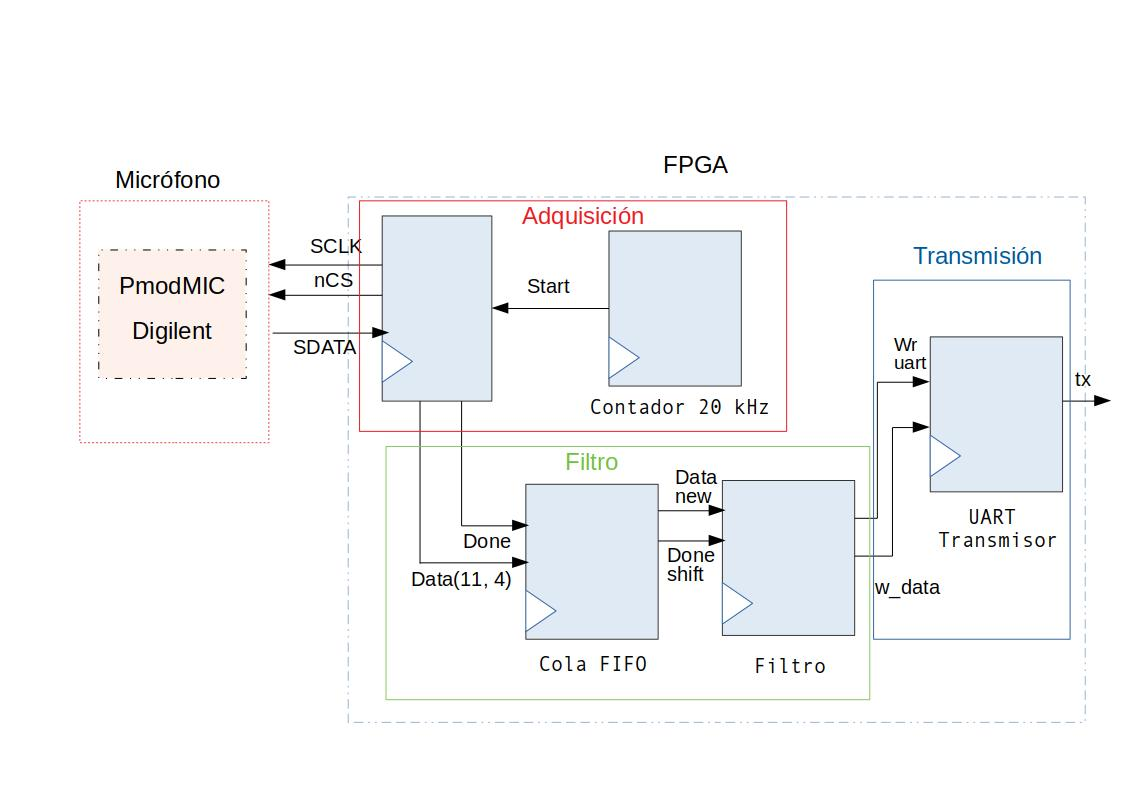
\includegraphics[width=0.7\linewidth]{conceptual.jpg}
    \caption{Esquema conceptual de la comunicación entre la FPGA y el microfono. La etapa de adquisición muestrea a 20 kHz los datos de audio que envia el microfono a traves de \texttt{SDATA}. El filtrado registra 20 de estos datos para realizar una convolución lineal. Por último, la trasmisión se realiza a través del puerto UART \texttt{tx} en forma serial}
    \label{fig:conceptual}
\end{figure}

En la FPGA se almacenan una serie de registros binarios \texttt{x[n]}, los cuales se convolucionan en cada muestreo con los coeficientes del filtro digital \textit{h[n]}, siguiendo la ecuación:

\begin{equation}
\centering
y[n]=\sum_{i=0}^{N}x[n]*h[n-i] 
    
\end{equation}

La FPGA realiza un muestreo de los datos del micrófono con una frecuencia de 20 kHz, mientras que el reloj interno de la misma para procesar cada muestra \textit{y[n]} posee una frecuencia de 100 MHz. 

\section{Implementación modular y pruebas}

La implementación del microfono en la FPGA consta de tres etapas: adquisición, filtrado y transmisión.


\subsection{Adquisición}

Para muestrear los datos del micrófono, se utilizó un módulo en VHDL que comunica al microfono PmodMIC con la placa. Esta entidad es una maquina de estados secuencial que recibe 16 bits en serie del periférico, siendo 12 de ellos bits de datos y el resto en cero.

Se utilizó un contador que pone la señal \texttt{start} en alto con una frecuencia de 20 kHz para comenzar a recibir los datos en serie del periférico. El mismo cuenta 5000 pulsos del reloj de la placa (con una frecuencia de 100 MHz). Cuando finaliza el ciclo de recepción, el módulo devuelve los 12 bits de datos en paralelo junto con una señal de finalización.

\subsection{Filtrado}

El filtrado de la señal en tiempo real se basa en la interacción de dos módulos: una implementación del filtro lineal descripto en la \eqref{eq:filtro} y una cola FIFO(\textit{primero en entrar, primero en salir}.

Para verificar su correcto funcionamiento, el test bench \textit{Filtertest.vhd} simula una señal impulsiva \textit{d[n]} para verificar la respuesta al impulso del filtro lineal. También se envia una señal escalón, verificando que la selida resulta en la suma causal de los coeficientes del filtro.

\subsubsection{Filtro Lineal}

El filtro digital se basa en una maquina de estados(\ref{fig:filtro_fsmd}) que realiza el producto y la suma de 20 registros del micrófono con los coeficientes de la respuesta al impulso. 

\begin{figure}[H!]
  \centering
  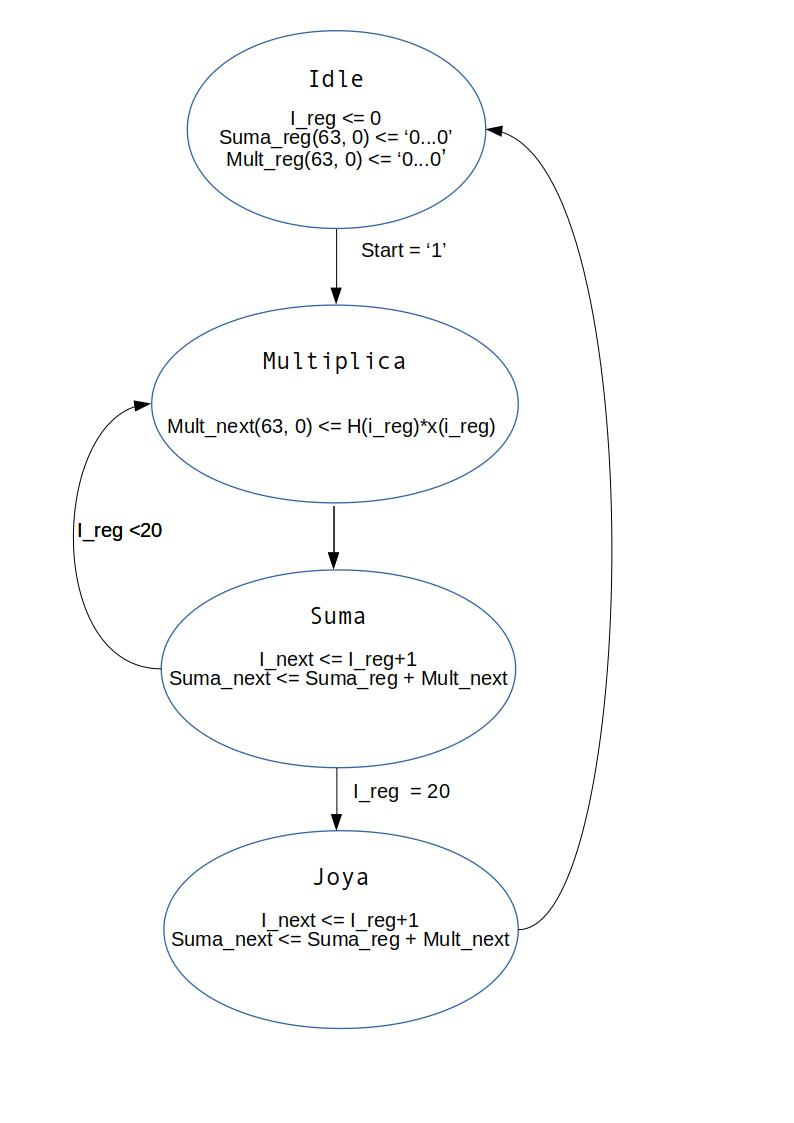
\includegraphics[width=0.6\linewidth]{filtro_fsmd.jpg}
  \caption{Maquina de estados del filtro lineal. }
  \label{fig:filtro_fsmd}
\end{figure}

Las operaciones utilizan una representación de punto fijo en complemento a dos(\ref{fig:operacion}). Esta notación destina 23 bits a la parte decimal, que corresponden a los coeficientes del filtro y 8 bits a la parte entera, correspondientes a cada dato binario de la señal. Se utilizan 8 de los 12 datos de información que entrega el micrófono. La multiplicación duplica la representación así como la posición del punto decimal. Al finalizar las operaciones se devuelve en paralelo 8 bits, correspondientes a la parte entera junto con la señal de finalización. 

\begin{figure}[H]
  \centering
  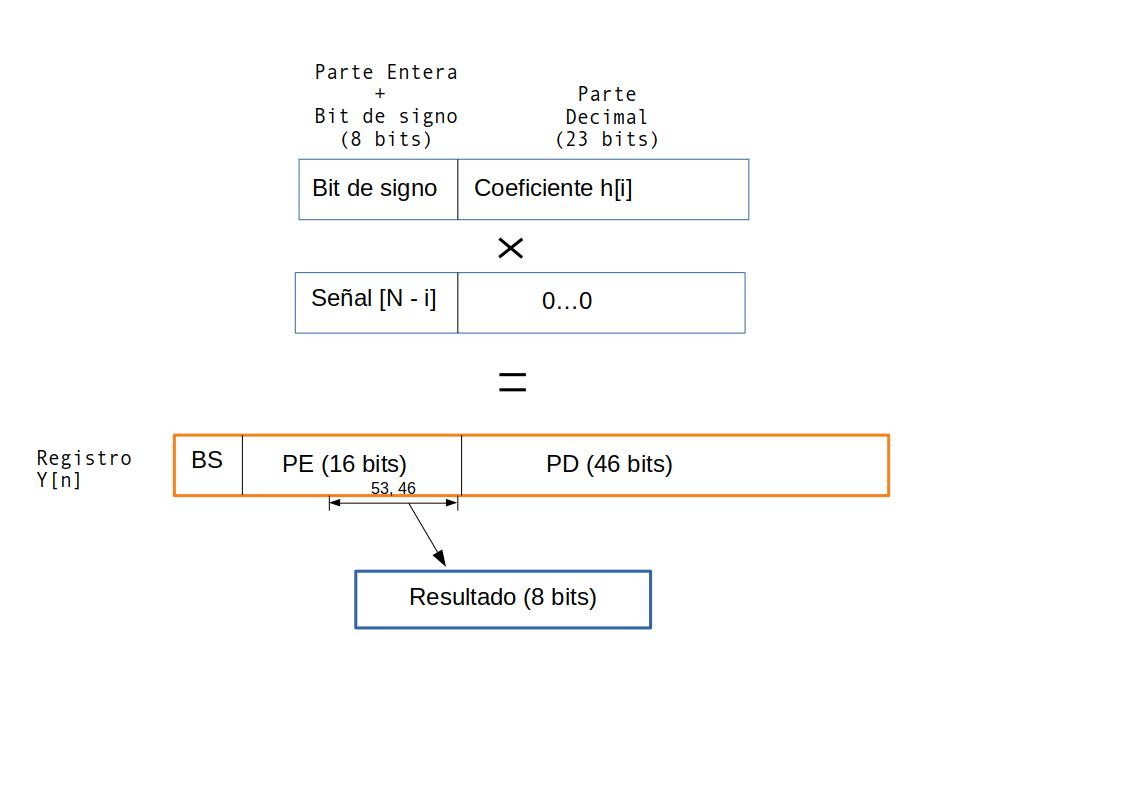
\includegraphics[width=0.8\linewidth]{filtro_op.jpg}
  \caption{Operación del filtro en aritmética de punto fijo. Cada uno de los coeficientes del filtro pasa bajos es representado en la parte decimal(extendido en la parte entera con su bit de signo) y multiplicado por los datos digitales, ubicados en la parte entera(extendido en la parte decimal con ceros). El producto de ambos tiene el doble de precisión y el resultado de la convolución se encuentra en los primeros 8 bits de su parte entera.}
  \label{fig:operacion}
\end{figure}


\subsubsection{Cola FIFO}

Los datos adquiridos por el micrófono deben ser almacenados para poder realizar el filtrado explicado previamente. Dado que para muestra filtrada \texttt{y[n]} se requieren de los 20 previos registros digitales, se implementó una cola FIFO, cuya lógica elimina los primeros datos que ingresan al registro y adjunta los nuevos datos de audio(\ref{fig:fifo_reg}). 

\begin{figure}[H]
  \centering
  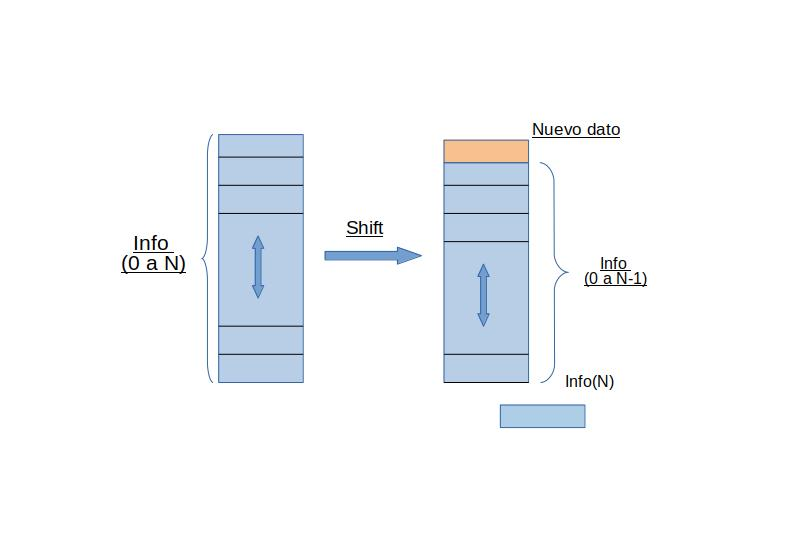
\includegraphics[width=0.8\linewidth]{cola_fifo.jpg}
  \caption{Funcionamiento de la cola FIFO. Al ingresar un nuevo dato, el mismo se adjunta al principio de la cola, eliminando el registro más viejo de la misma.}
  \label{fig:fifo_reg}
\end{figure}

\subsection{Transmisión}

Las muestras filtradas se transmiten mediante un dispositivo UART presente en la FPGA, que toma bytes de datos y envía cada uno de los bits en forma secuencial. Se utiliza una unidad de transmisión que acuerda el 'baudrate'(400800), las señales por segundo enviadas y los bits de parada de cada byte transmitido. Además, posee una cola FIFO que puede registrar datos a enviar en el caso de una transmisión más lenta. 

Para su prueba, se utilizó un contador hexadecimal, con rango cíclico de 00 a FF, enviando cada uno de estos datos a través de la UART hacia una terminal serial. 


\section{Implementación integral y resultados}

Se integraron las tres etapas del sistema en un módulo principal en VHDL. Se adquirieron dos señales de audio para verificar el funcionamiento del filtrado. La \ref{fig:freq_sweep} muestra el espectro filtrado de un barrido en frecuencia desde 1 kHz hasta 10 kHz, mientras que la \ref{fig: freq_sum} es la respuesta ante una suma de armónicos de 1 kHz. 

\begin{figure*}[h!]
    \centering
    \begin{subfigure}[Espectro de la señal filtrada]
        \centering
        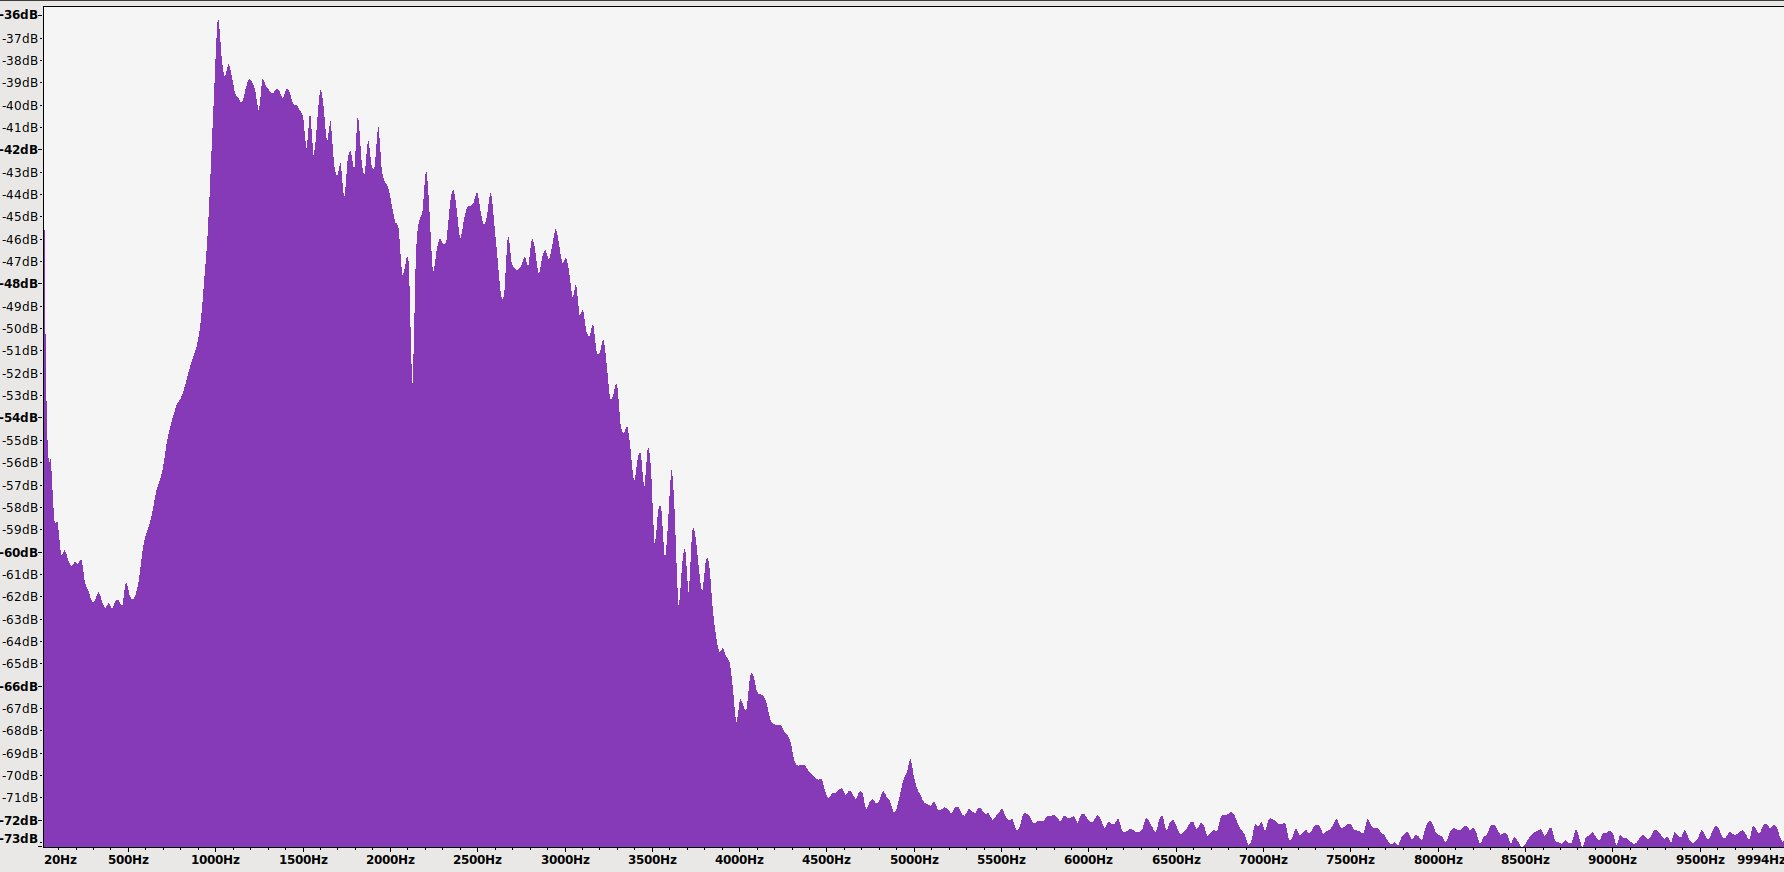
\includegraphics[width=0.45\linewidth]{Freq_sweep.jpg}
    \end{subfigure}
    
    \begin{subfigure}[Espectro de la señal original]
        \centering
        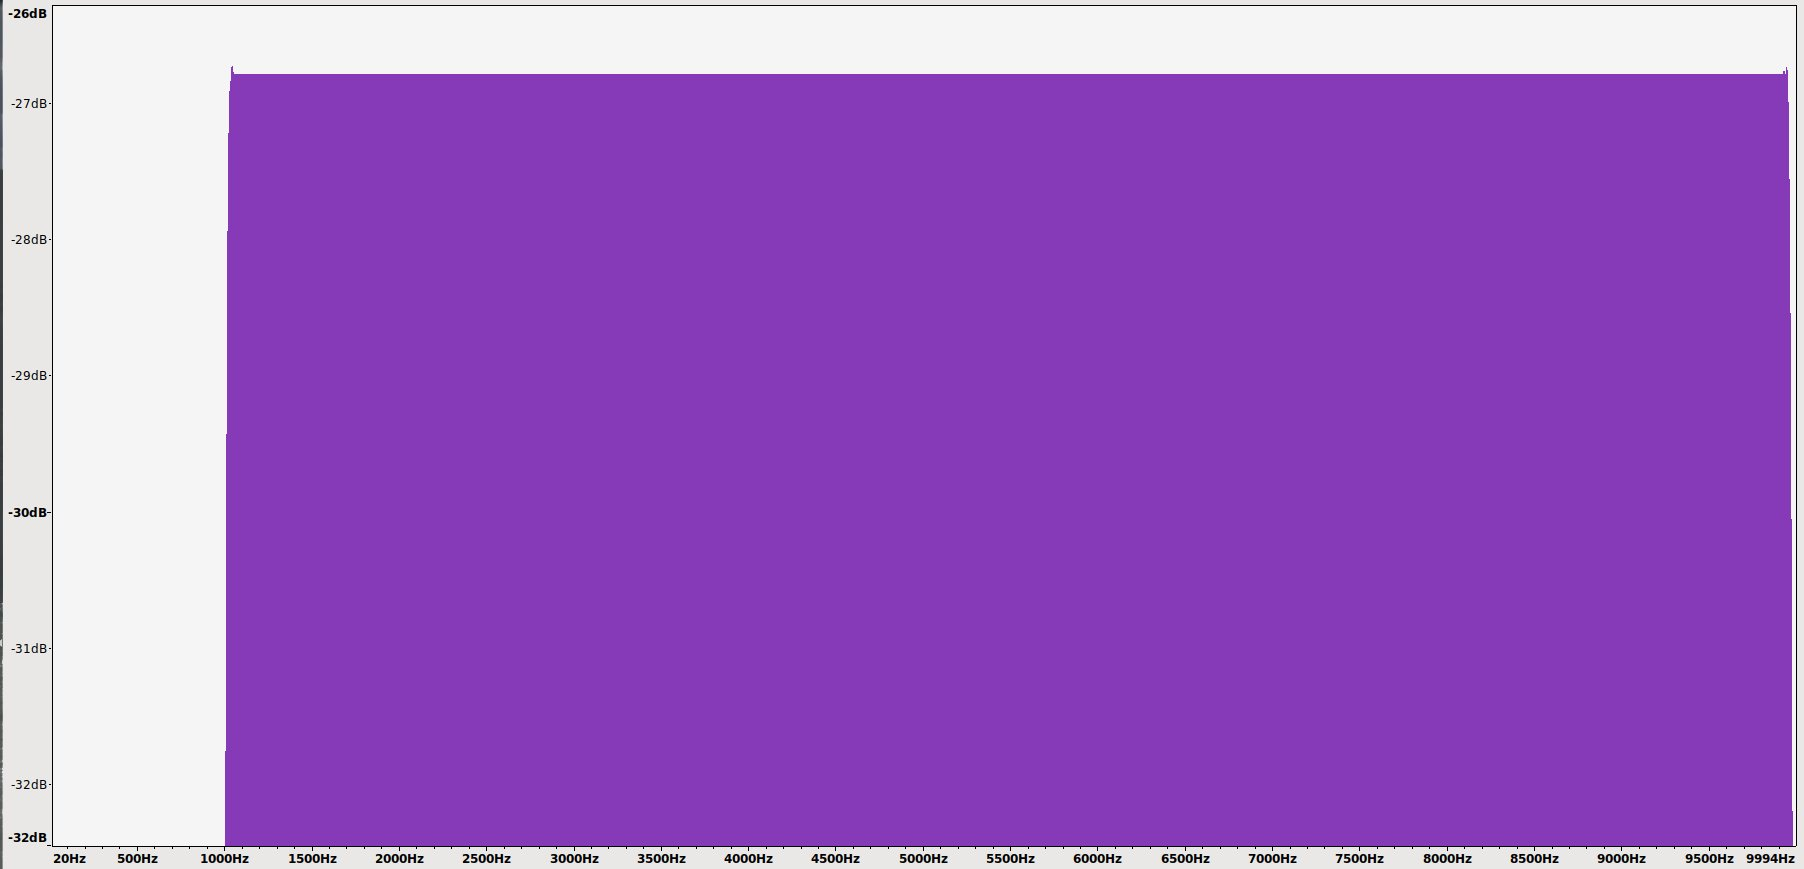
\includegraphics[width=0.45\linewidth]{Orig_sweep.jpg}
    \end{subfigure}
    \caption{Barrido en frecuencia}
\end{figure*}

\begin{figure*}[h!]
    \centering
    \begin{subfigure}[Espectro de la señal filtrada]
        \centering
        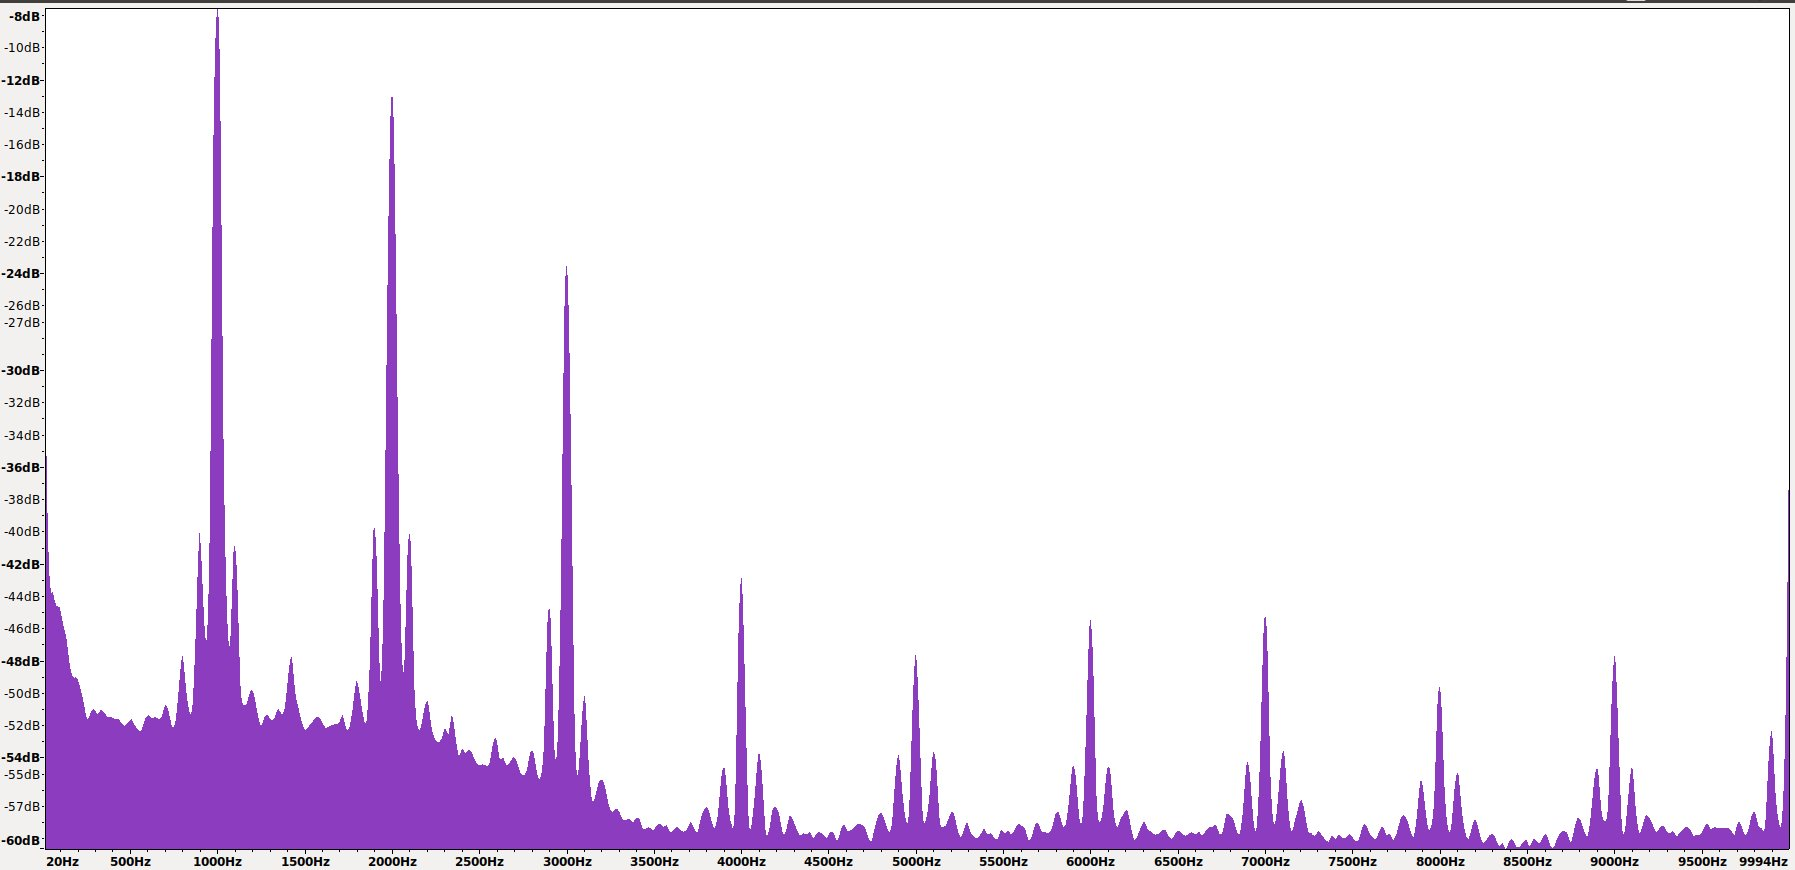
\includegraphics[width=0.45\linewidth]{Suma_tonos.jpg}
    \end{subfigure}
    
    \begin{subfigure}[Espectro de la señal original]
        \centering
        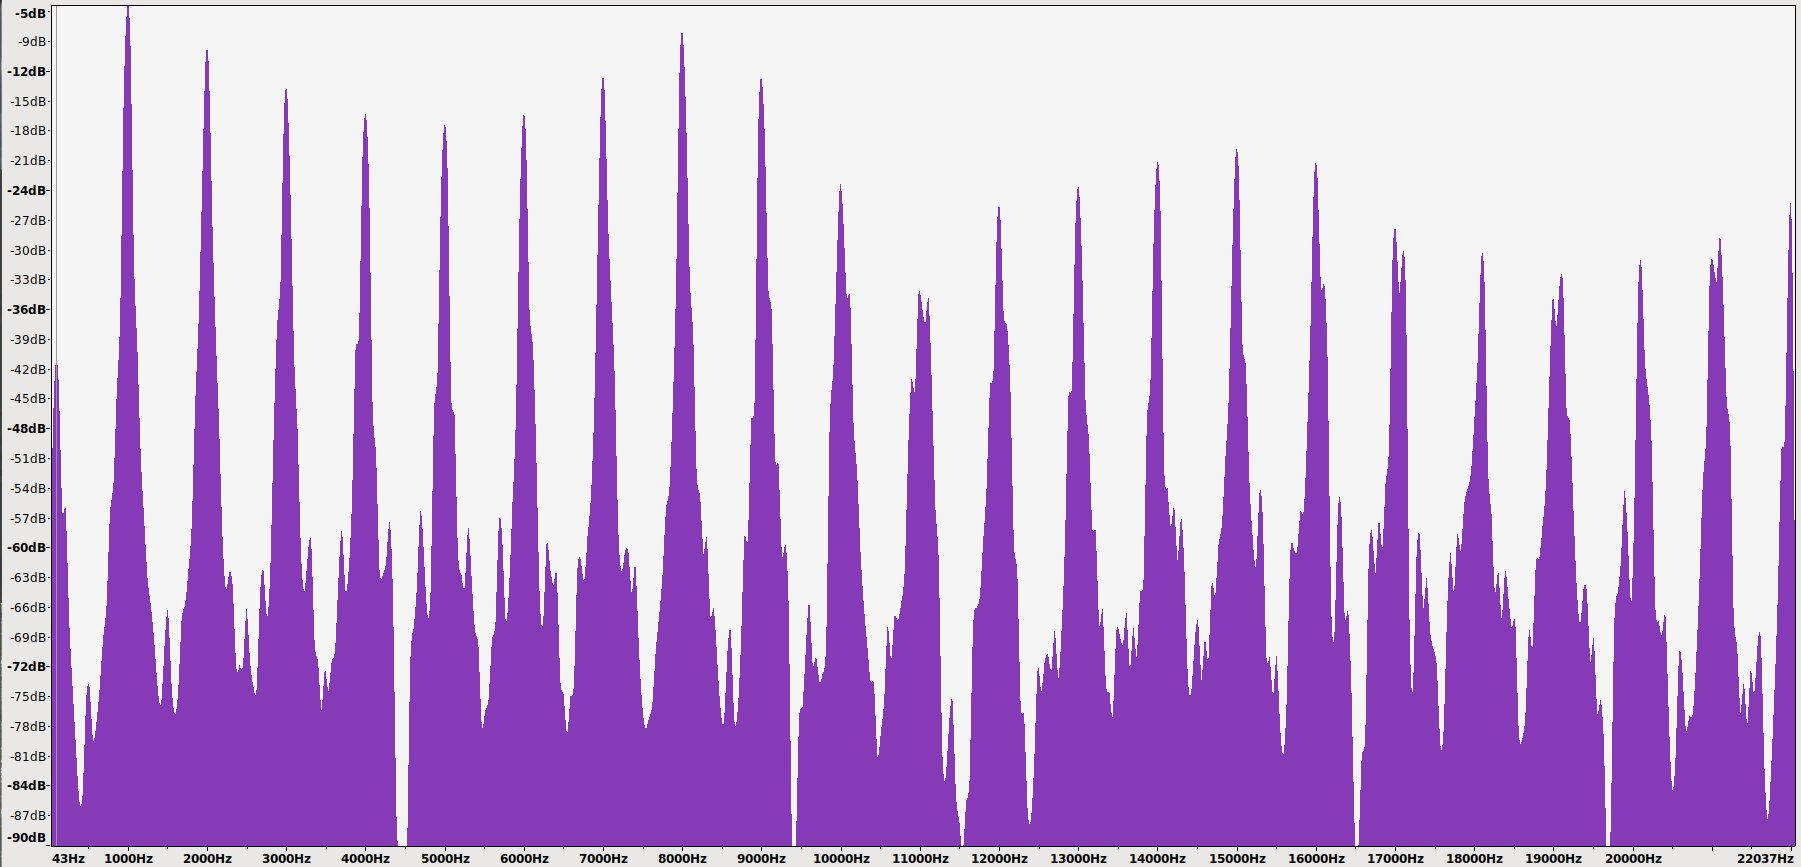
\includegraphics[width=0.45\linewidth]{suma_orig.jpg}
    \end{subfigure}
    \caption{Suma de tonos armónicos de 1 kHz}
\end{figure*}

\section{Conclusiones}

Se implementó un sistema de adquisición, filtrado y transmisión de datos digitales de audio en una FPGA con un micrófono periférico. Se utilizó un filtro de respuesta finita al impulso triangular de 20 coeficientes, operando con una representación de punto fijo. Se verificó que el filtro pasabajos realiza una atenuación a partir de la frecuencia de corte de 4 kHz


\begin{thebibliography}{}
	%% Apellido, Nombre; Apellido, Nombre; etc; Nombre del texto; Edición; Nombre del editor.
	\bibitem{1}{\url{https://github.com/marcoso96/Estacionamiento}}
    \bibitem{2}{Chu, Pong P. \textit{FPGA Prototyping by VHDL Examples}}
    
\end{thebibliography}
\end{document}